\chapter*{Funkcjonalność projektu}
Projekt jest wysoce wyspecjalizowany -- aplikacja przeprowadza wyłącznie proces symulacji i uczenia. Użytkownik może konfigurować ustawienia tego procesu.
\section*{Wymagania funkcjonalne}
\begin{itemize}
	\item Przeprowadzenie procesu uczenia optymalnych czasów świecenia sygnalizatorów na skrzyżowaniu za pośrednictwem algorytmu ewolucyjnego,
	\item Konfiguracja ustawień symulacji, będącej bazą procesu uczenia,
	\item Konfiguracja ustawień algorytmu ewolucyjnego,
	\item Wyświetlanie na bieżąco informacji o przebiegu uczenia ,
	\item Wyświetlenie wyników uczenia po jego zakończeniu.
\end{itemize}
\section*{Wymagania pozafunkcjonalne}
\begin{itemize}
	\item Stabilność -- aplikacja musi pracować bezawaryjnie przez wiele godzin,
	\item Wydajność -- aplikacja musi działać na tyle wydajnie, aby symulacja mogła być przeprowadzana kilkadziesiąt razy szybciej niż czas rzeczywisty.
\end{itemize}
\begin{figure}
	\centering
	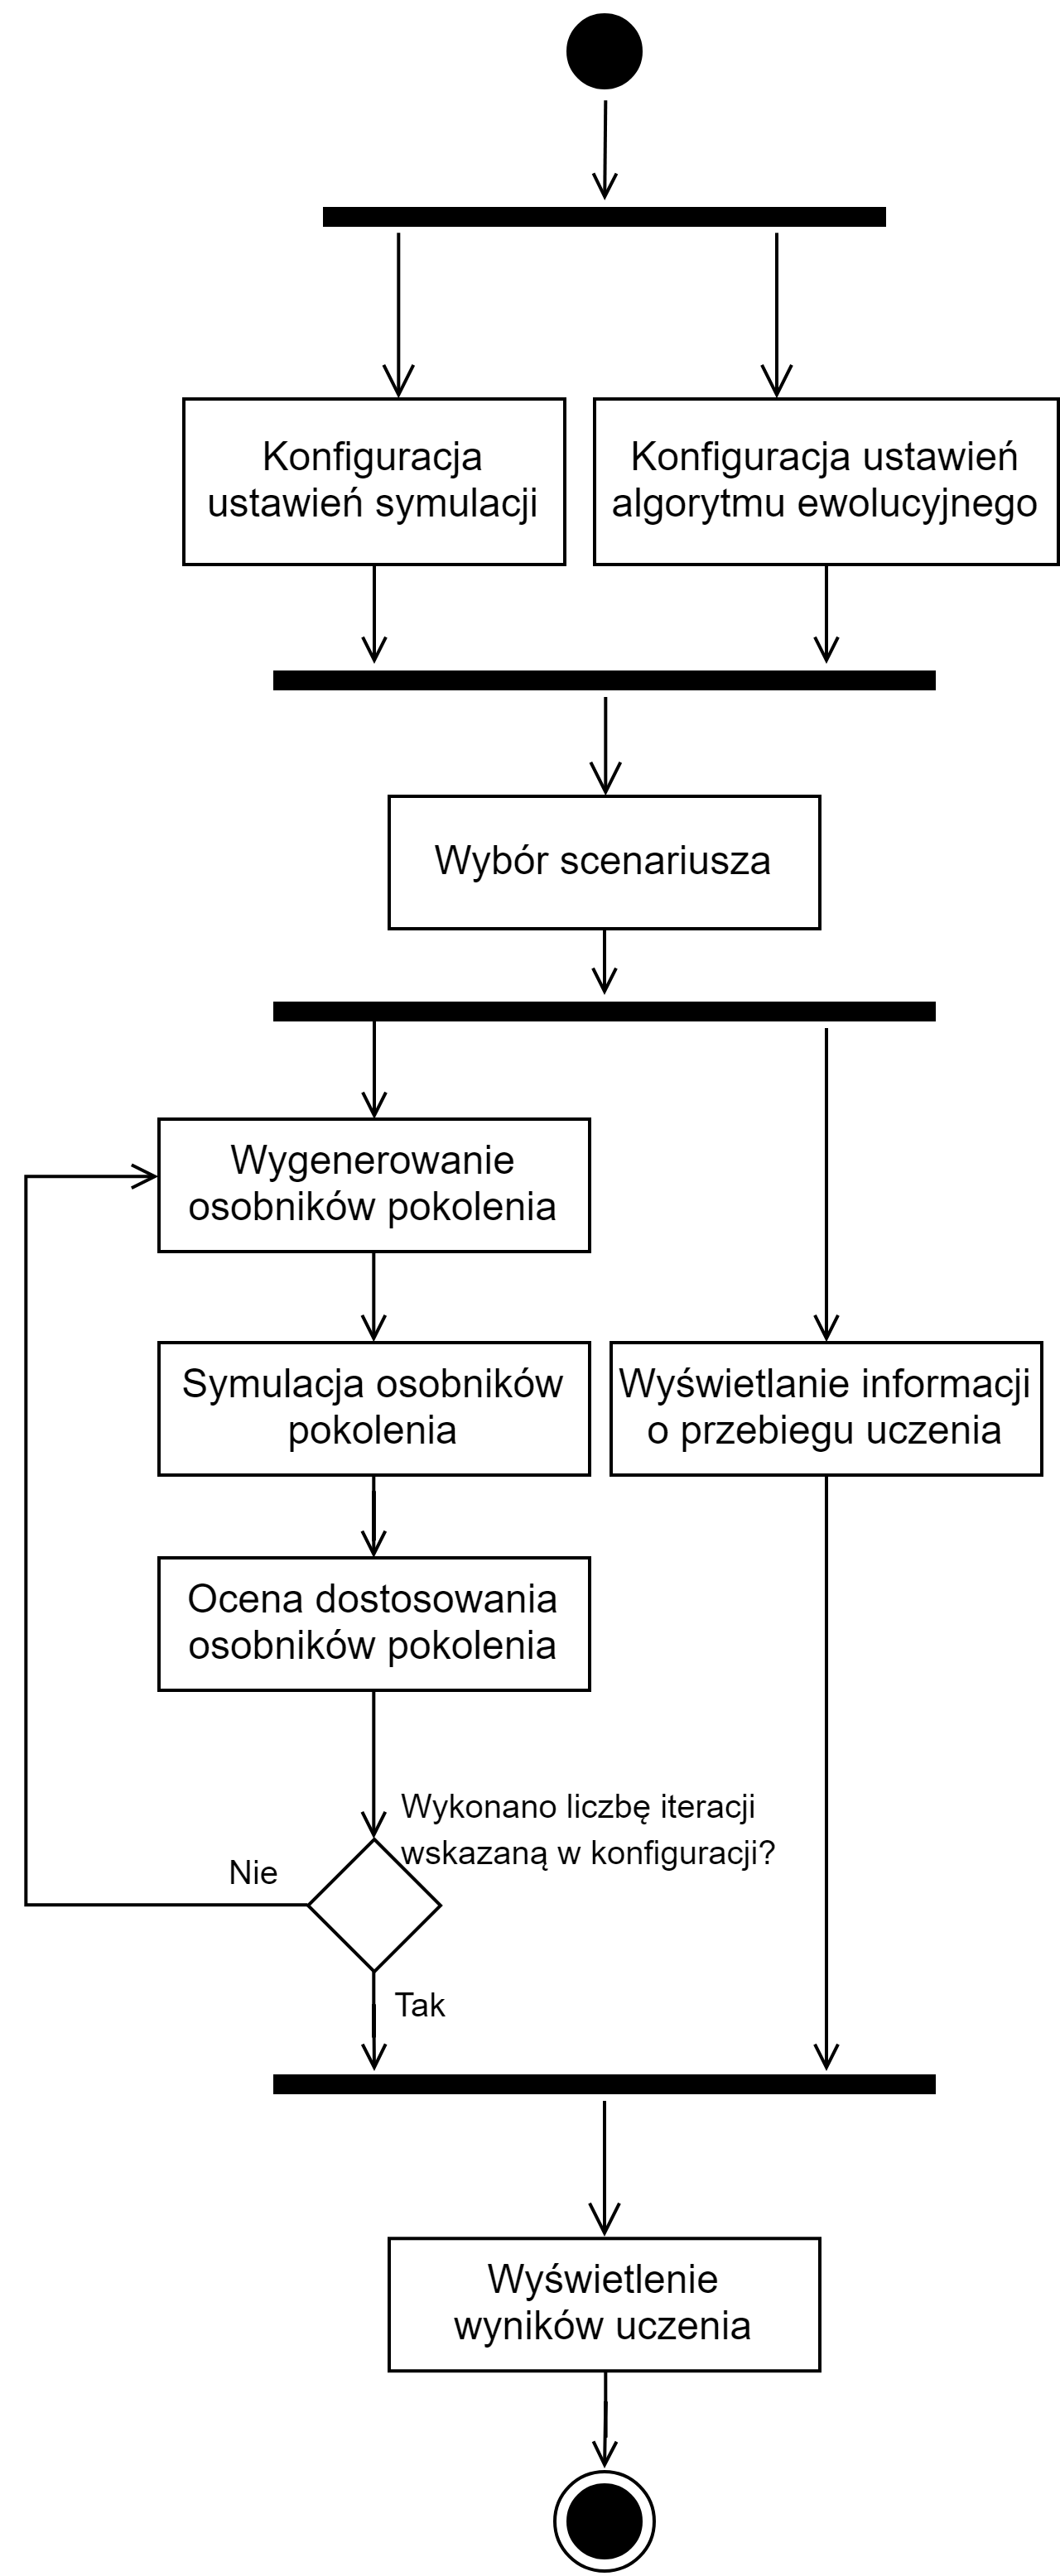
\includegraphics[height=0.9\textheight]{diagram_aktywnosci}
	\caption[Diagram aktywności przypadku użycia ,,Przeprowadź proces uczenia sygnalizacji'']{Diagram aktywności przypadku użycia ,,Przeprowadź proces uczenia sygnalizacji''}
	\label{fig:diagramaktywnosci}
\end{figure}
\section*{Przypadki użycia}
W projekt występuje tylko jeden przypadek użycia: ,,Przeprowadź proces optymalizacji sygnalizacji świetlnej''. Przedstawia go diagram aktywności na rysunku~\ref{fig:diagramaktywnosci} oraz (hm)~\ref{tab:scenariusz}.
\begin{table}
	\caption{Scenariusz przypadku użycia ,,Przeprowadź proces optymalizacji sygnalizacji świetlnej''}
	\begin{tabularx}{\textwidth}{|l|X|}
		\hline 
		Nazwa & Przeprowadź proces optymalizacji sygnalizacji świetlnej \\ 
		\hline 
		Aktorzy & Użytkownik \\ 
		\hline 
		Opis & Funkcja pozwala użytkownikowi wywołać proces optymalizacji sygnalizacji świetlnej na skrzyżowaniu \\ 
		\hline
		Warunki początkowe & brak \\
		\hline 
		Główny przepływ zdarzeń & 1. Użytkownik wprowadza w menu głównym aplikacji ustawienia. \newline 
		1.1 Użytkownik wprowadza ustawienia symulacji \newline
		1.2 Użytkownik wprowadza ustawienia algorytmu ewolucyjnego \\ 
		\hline
		Warunki końcowe & Zakończono proces optymalizacji i wyświetlono wyniki uczenia \\
		\hline
	\end{tabularx} 
	\label{tab:scenariusz}
\end{table}
